\chapter{Code Description}
\section{Code Overview}
The code we used is called SLH (Seven League Hydro). It was originally developed by Dr. Fabian Miczek during his PhD thesis (2013). SLH is a finite-volume multidimensional code that solves Euler equations (ideal hydrodynamic) using explicit or implicit methods. The advantage of implicit methods lies in the fact that the time step is constantly redefined optimizing computational resources using the so called cfl criterion for numerical stability. In this case a non-linear system of equations is solved using the Newton-Ralphson method, in which at every time step a linear system is solved through the Krylov subspace methods. The efficiency of all these computational methods is strongly dependent on the type of linear system solved and the cluster architecture used. 

From the point of view of simulation domain SLH allows us to implement a general curvilinear grid instead of a simple Cartesian one by defining a metric, the elements of which are needed to correctly compute the fluxes at the cells interfaces. The code decomposes automatically the domain to parallelize the computation on the desired number of processors, using MPI and openMP. A wide choice of boundary conditions are implemented. 

Furthermore SLH implements a general equation of state, a nuclear reaction network, passive and active scalars which are fundamental for the study of the chemical composition of the fluid, radiation in the diffusion limit and thermal conduction. 

Over the years SHL has undergone several scaling tests, the most remarkable of which at the Jülich Supercomputing Center (JSC) in 2016 where it scaled over all the $458752$ cores of \textit{JUQUEEN} (a Blue Gene machine, currently the last generation of IBM supercomputers).

\section{Finite Volume Discretization}
In order to discretize the physical domain we employ a set of curvilinear coordinates $\xi, \eta, \zeta$. This set is partitioned by a regular, equidistant grid which $N_{\xi} \times N_{\eta} \times N_{\zeta}$ cells. Without loss of generality, we define the domain extent such that
\begin{equation}
\begin{split}
\xi \in [1/2, N_{\xi} + 1/2] \\
\eta \in [1/2, N_{\eta} + 1/2] \\
\zeta \in [1/2, N_{\zeta} + 1/2] 
\end{split}
\end{equation}
We are hence here imposing that the cells volume is constant, i.e. $\Delta \xi = \Delta \eta = \Delta \zeta = 1$ in order to simplify some calculations. This might in general not be the case, since SLH allows the user to call a general curvilinear grid. In this particular case integer values of coordinates refer to cell centers, half integer to cell faces, e.g. by $(\xi, \eta, \zeta) = (i, j + 1/2, k)$ we refer to the interface at the right-hand side of cell $(i, j, k)$.

Both for analytic and numerical study of Euler equations, it is useful to switch to a dimensionless workframe. This is achieved by decomposing state variables into two parts, namely a reference value (denoted with an $r$) and a dimensionless number (denoted with a hat), e.g. $\rho = \rho_r \cdot \hat{\rho}$. This leads to a state vector 
\begin{equation}
\frac{\partial \mathbf{\hat{U}}}{\partial \hat{t}} + \frac{\partial \mathbf{\hat{F}}_x}{\partial \hat{x}} + \frac{\partial \mathbf{\hat{F}}_y}{\partial \hat{y}} + \frac{\partial \mathbf{\hat{F}}_z}{\partial \hat{z}} = \mathbf{\hat{S}}
\end{equation}
where the quantities $\mathbf{\hat{U}}$, $\mathbf{\hat{F}}_x$, $\mathbf{\hat{F}}_y$ and $\mathbf{\hat{F}}_z$ are defined by the stress-energy tensor as discussed in the previous chapter. From now on for simplicity we will drop the hat notation. We discretize \textit{in space} Euler equation as 
\begin{equation}
J^{-1}\frac{\partial \mathbf{U}}{\partial t} + \nabla_{\xi, \eta, \zeta} \cdot \mathbf{F} = J^{-1} \mathbf{S}
\end{equation}
where $J$ is the determinant of the Jacobian of the transformation from the physical domain to the computational grid.

These equations are integrated over the volume $\Omega_{i, j, k} = \Delta \xi \times \Delta \eta \times \Delta \zeta $ of the cell $(i, j, k)$, which in our assumptions is constant for every cell (differentially $d \Omega = d \xi \times d \eta \times d \zeta$) of the cell $(i, j, k)$.
\begin{equation}
	\int_{\Omega_{i, j, k}} J^{-1} \frac{\partial \mathbf{U}}{\partial t} d \Omega + \int_{\Omega_{i, j, k}} \nabla_{\xi \eta \zeta} \cdot \mathbf{F} d\Omega = \int_{\Omega_{i, j, k}} J^{-1} \mathbf{S} d \Omega
\end{equation}

By exchanging the derivatives with the integrals, it is clear that these are nothing but the average of the conserved quantities in the cell times the volume of it. We may therefore introduce some new cell-averaged quantities such as 
\begin{equation}
\mathbf{U}_{i, j, k} = \int_{\Omega_{i, j, k}} J^{-1} \mathbf{U} d \Omega \qquad \mathbf{S}_{i, j, k} = \int_{\Omega_{i, j, k}} J^{-1} \mathbf{S} d \Omega
\end{equation}
In addition to this, we can apply Gauss theorem on the second term on the self-hand side and obtain the following expression
\begin{equation}
	\frac{\partial \mathbf{U}_{i, j, k}}{\partial t} + \frac{1}{V_{i, j, k}} \oint_{\partial \Omega} \mathbf{F} \cdot d \mathbf{s} = \mathbf{S}_{i, j, k}
\end{equation}
If we suppose to know the integral fluxes through the six interfaces, we can further decompose the second term into six numerical fluxes as follows
\begin{equation}
\begin{split}
	\mathbf{F}_{i+ 1/2, j, k} = \oint_{\partial \Omega_{(i + 1/2, j, k)}} \mathbf{F}_{\xi} d \xi \\
	\mathbf{F}_{i, j + 1/2, k} = \oint_{\partial \Omega_{(i , j + 1/2, k)}} \mathbf{F}_{\eta} d \eta \\
	\mathbf{F}_{i, j, k + 1/2} = \oint_{\partial \Omega_{(i , j, k + 1/2)}} \mathbf{F}_{\zeta} d \zeta \\
\end{split}
\end{equation}
This allows us to write down the discretized Euler equations as 

\begin{equation}
\begin{split}
	\frac{\partial \mathbf{U}_{i, j, k}}{\partial t} + \frac{1}{V_{i, j, k}} ( & \mathbf{F}_{i + 1/2, j, k} + \mathbf{F}_{i - 1/2, j, k} +\mathbf{F}_{i , j + 1/2, k} + \\
	& \mathbf{F}_{i , j - 1/2, k} +  \mathbf{F}_{i , j, k + 1/2} + \mathbf{F}_{i , j, k - 1/2}) = \mathbf{S}_{i, j, k}
\end{split}
\end{equation}
What is stored in the memory are the cell-averaged quantities. Their value changes only by numerical fluxes from the neighbor cells or by source terms. This implies that, if there are no source terms, the sum of cell-averaged variables cannot change. In this way, the finite volume discretization perfectly reflects the conservative nature of Hydrodynamic. We would like to underline that the numerical fluxes still remain unknown, and should be reconstructed for the cell $(i, j, k)$ from the surrounding cells. In addition to that, what we performed was a \textit{partial discretization}, since in time we still have a continuous time derivative and no finite difference. This method, through which we discretize first the spatial dimension and then separately the temporal one, is known as \textbf{method of lines}. It is a very effective method to reduce partial differential equations to a set of coupled ordinary differential equations such as
\begin{equation}\label{eq:methodoflines}
	\frac{\partial \mathbf{U}_{i, j, k}}{\partial t} + \mathbf{R}_{i, j, k}=0
\end{equation}
where the vector $\mathbf{R}_{i, j, k}$ is known as \textit{spatial residual} of the cell $(i, j, k)$. As previously mentioned, this is a function with the numerical fluxes of the surrounding cells, and suitable numerical methods are needed in order to correctly compute them.
\section{Explicit vs. Implicit Time Stepping}
The simplest way to discretize in time equation \ref{eq:methodoflines} is the so called \textbf{forward Euler method} \footnote{The forward Euler method can be applied to resolve general PDEs, not only Euler equations. It is a coincidence that both the fluid dynamics equations and the numerical scheme that we use to solve them were discovered by swiss mathematician Leonhard Euler.}:
\begin{equation}\label{eq:forwardeuler}
	\frac{\mathbf{U}^{n+1}_{i, j, k} - \mathbf{U}^{n}_{i, j, k}}{\Delta t} + \mathbf{R}_{i, j, k}(\mathbf{U}^n)=0
\end{equation}
This method simply approximates the time derivative with a finite difference at each grid point, and the spacial residual is evaluated at the old time step. Notice that equation \ref{eq:forwardeuler} can be solved analytically for the conserved quantity $\mathbf{U}^{n+1}_{i, j, k}$. This means that we are dealing with an \textit{explicit time stepping}. Although equation \label{eq:forwardeuler} has a very direct and simple implementation, this method is first-order accurate i.e. it has an approximation error that is $\mathcal{O}(\Delta t)$.

A considerable amount of higher-order explicit time stepping schemes are available. In SLH the so-called third-order Runge-Kutta scheme (RK3) developed by Shu and Osher (1988) is implemented. 

The advantages of an explicit time stepping method are essentially two: they are easy to implement and they require little resources memory wise on the hardware. The biggest disadvantage is that one always has to choose the time step lower than a maximum value $\delta t$. In case this condition is not fulfilled, numerical errors start to grow over time and dominate over the physical solution. In the case of Euler equation, in order to determine $\delta t$, the CFL criterion is generally used
\begin{equation}\label{eq:cfl}
	\Delta t = \frac{\mathrm{CFL}}{N_{\mathrm{dim}}}\mathrm{min} \left(  \frac{\Delta x}{|q_n| + c/M}   \right)
\end{equation}
where $N_{\mathrm{dim}}$ is the number of dimensions, $\Delta x$ is the cell width, the quantity at denominator is the wave velocity and the minimum has to be intended over all the computational grid. At last CFL is a dimensionless coefficient that determines how many cells a wave can travel for time step. For all the explicit time steppers implemented in SLH, CFL is always smaller than unity. Roughly one can see that $\Delta t \propto M$, hence the lower the mach number, the lower the maximum allowed time step. This criterion shows why the use of explicit time steppers for low mach flow is computationally impracticable.
For this reason we rely on a new discretization method, namely the \textbf{backward Euler method}. According to this discretization the conserved quantities at the time step $n+1$ are given by
\begin{equation}\label{eq:backward}
	\frac{\mathbf{U}^{n+1}_{i, j, k} - \mathbf{U}^{n}_{i, j, k}}{\Delta t} + \mathbf{R}_{i, j, k}(\mathbf{U}^{n+1})=0
\end{equation}
The only difference compared to the forward Euler method is that the residual is evaluated at the time step $n+1$ instead of $n$. An analytic solution for this equations is hence in general not possible, and sophisticated numerical solvers need to be employed in order to find an approximate solution (in our case we implement the so-called \textbf{Newton-Raphson method}, see next section). The advantage of integrating implicitly is very well explained by figure \ref{fig:implicit}. What is shown is a slow advection wave with a relatively low frequency, with a high frequency acoustic wave on it. Suppose to start from $t=0$ integrating explicitly with the forward Euler method. Since the derivative is evaluated at $t=0$, the risk is that the acoustic wave completely dominates the result, leading to a corrupted value for the conserved quantity. Integrating implicitly instead, the derivative is evaluated over the entire time step. In other words we extrapolate the derivative starting from the final point backward to the initial one, ensuring that the finite difference method resolves the phenomena at the time scale we are interested in. Acoustic waves in the low mach regime in fact decouple from the advective solution, hence we don't need to resolve them. The backward Euler method again generates an error which is $\mathcal{O}(\Delta t)$, but more refined methods are available in the literature and are implemented in SLH. 

\begin{figure}[t]
\centering
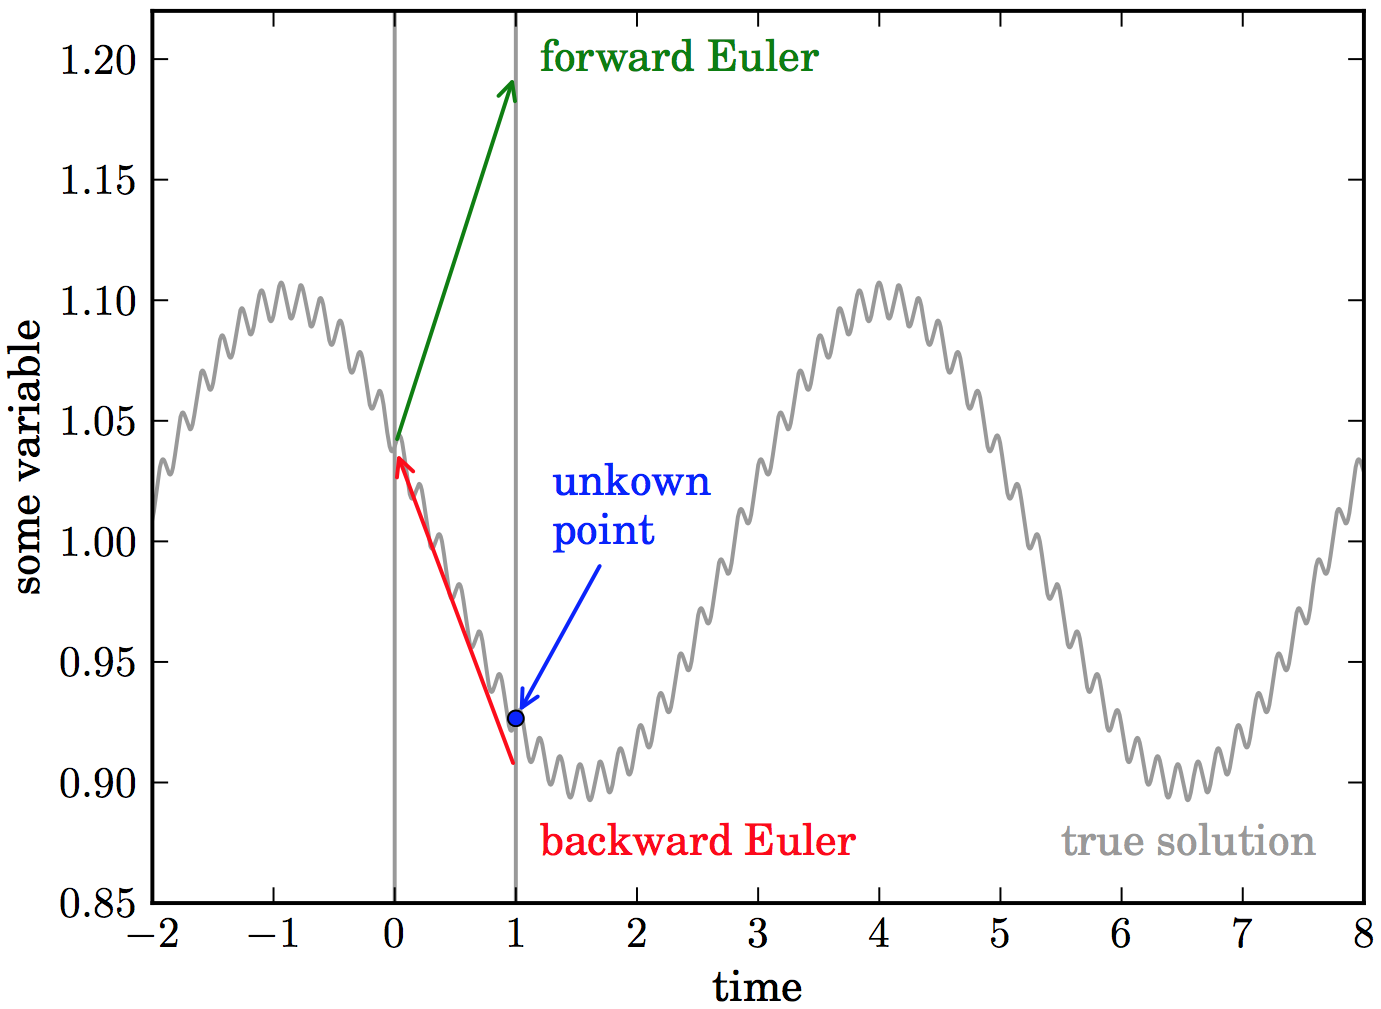
\includegraphics[width=10cm]{./img/implicit}
\caption{Conceptual difference between explicit and implicit integration. Picture from Miczek, 2013.}
\label{fig:implicit}
\centering
\end{figure}
The question we need to answer when choosing the integration technique is if the rise in efficiency given by implicit methods compensate the loss, given by the expensive numerical solvers needed to approximate the solution of the implicit equation. In the low mach regime (from $M \simeq 10^{-4}$ to $10^{-3}$) an implicit integration with SLH is always more convenient. 

\section{Newton-Raphson Method}
In this section we analyze the so-called \textbf{Newton-Raphson method}, which is the iterative solver implemented in SLH in order to find an approximate solution to the implicit equation \ref{eq:backward}. The first step we need to take is to move every term of our discretized equation to the left-hand side and define a quantity $\mathbf{D}_{i, j, k}(\mathbf{U}^{n+1})$ called \textit{defect}
\begin{equation}\label{eq:defect}
	\mathbf{D}_{i, j, k}(\mathbf{U}^{n+1}) = \mathbf{R}_{i, j, k}(\mathbf{U}^{n+1}) + \frac{\mathbf{U}_{i, j, k}^{n+1}}{\Delta t} - \frac{\mathbf{U}^n_{i, j, k}}{\Delta t} = 0
\end{equation}
Obviously the equations are solved if the defect is zero. This algorithm starts from an initial guess $\mathbf{U}^0$, which is iteratively refined by calling
\begin{equation}\label{eq:newtonraphson}
	\mathbf{U}^{k+1} = \mathbf{U}^k - \left( \lambda \frac{\partial \mathbf{D}^k}{\partial \mathbf{U}}  \right)^{-1} \mathbf{D}^k
\end{equation}
Where $\lambda$ is a convergence parameter that in generally set to one (in pathological cases it might be set $\lambda > 1$ to dump the convergence ratio). The more the iterations, the closer $\mathbf{U}^k$ gets to the root of $\mathbf{D}$.

In order to compute the right-hand side, one should invert the Jacobian of the defect, but this is computationally and memory wise very expensive. It is instead easier to rewrite \ref{eq:newtonraphson} as 
\begin{equation}
	\lambda \frac{\partial \mathbf{D}^k}{\partial \mathbf{U}} \Delta \mathbf{U} = - \mathbf{D}^k
\end{equation}
where $\Delta \mathbf{U}=\mathbf{U}^{k+1} - \mathbf{U}^k$. This is a very effective method to transform a system of non-linear equations to a set of systems of linear equations.

The Newton-Raphson method generally converges quadratically to the solution, i.e. the number of significant digits doubles at every iteration. In particular cases like a double root (namely $f'(\alpha)$=0, where $\alpha$ is the defect root) the convergence is linear. Obviously the first and second derivative should be non-zero over the iterative domain and to improve the efficiency the initial guess should be as close as possible to the root of the defect. In SLH we choose as $\mathbf{U}^0$ the solution of the previous time step.

SLH prints in the log file information about every iteration of the Newton-Raphson method for every variable. Specifically it prints the $\mathrm{L2}$ norm of the defect. For the density $\rho$ for instance
\begin{equation}\label{eq:l2defect}
	||\mathbf{D}||^{\rho} = \sqrt{ \sum_{i, j, k} \left( \mathbf{D}^{\rho}_{i, j, k}  \right)^2}
\end{equation}
which is the quantity that decreases quadratically.

In equation \ref{eq:defect} the very last term is a constant vector, since it's the state vector at the previous time step ($t=n$). Only the state vector at the current time step ($t=n+1$) changes at every iteration of the Newton-Raphson method. This is of course cause of numerical cancellation error. For this reason in SLH the $\mathrm{L2}$ norm of the defect is actually scaled by the $\mathrm{L2}$ norm of the constant vector, in order to monitor the convergence relative to machine precision \footnote{Recall that for double precision floating point value, machine precision is $\simeq 10^{-16}$}
\begin{equation}
	\frac{||\mathbf{D}||^{\rho}}{||\mathbf{U}^n / \Delta t||^{\rho}}
\end{equation}
In addition by scaling the defect $\mathrm{L2}$ norm, the convergence is monitored dimensionless.

Note that reaching machine precision when converging is actually rarely possible because of
\begin{itemize}
	\item{round-off errors in the discretization in the flux functions and in the linear solvers}
	\item{approximations in the defect Jacobian and in the linear systems}
\end{itemize}
Moreover, the process of discretization of Euler equations generates errors which depend on the numerical scheme and the grid. As a consequence, converging to machine precision might be a waste of computational resource.
